\documentclass[a4paper]{exam}

\usepackage{amsmath,amssymb, amsthm}
\usepackage{geometry}
\usepackage{graphicx}
\usepackage{hyperref}
\usepackage{xcolor}
\usepackage{wasysym}

\usepackage{xcolor}
\usepackage{wasysym}


\usepackage{tikz}
\usepackage{tikz-qtree}



\newtheorem{definition}{Definition}
\newtheorem{theorem}{Theorem}

\title{Weekly Challenge 04: Pumping Lemma}
\author{CS 212 Nature of Computation\\Habib University}
\date{Fall 2026}

\boxedpoints

\newcommand{\prob}{3-\textsc{coloring}} % Use this command to typeset the 3-coloring problem.

% \printanswers % Uncomment this line

\begin{document}
\maketitle

\begin{definition}
    Let $G =  (V,E)$ be a graph. A \emph{Coloring} of $G$ is a color assignment to vertices of $G$ such that no two adjacent vertices has the same color. More formally, a coloring is a function $C: V \to \mathbb{N}$ such that $\forall v, u \in V,\; \{u,v\} \in E \implies c(v)\neq c(u)$. 
\end{definition}

\begin{figure}[h]
    \begin{center}
    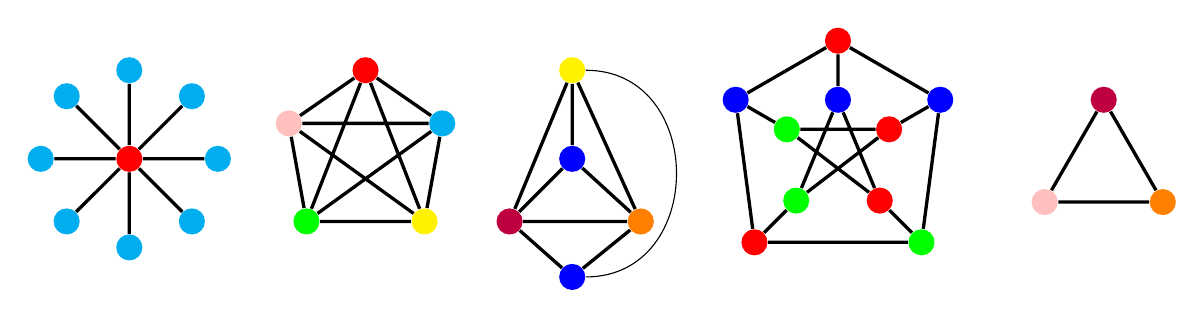
\begin{tikzpicture}[scale=.75]
        %star
        \node[style={fill=red,circle}] (1) at (0,0){};
        \node[style={fill=cyan,circle}] (2) at (0,1.5){};
        \node[style={fill=cyan,circle}] (3) at (1.5,0){};
        \node[style={fill=cyan,circle}] (4) at (-1.5,0){};
        \node[style={fill=cyan,circle}] (5) at (0,-1.5){};
        \node[style={fill=cyan,circle}] (6) at (1.06,1.06){};
        \node[style={fill=cyan,circle}] (7) at (-1.061,-1.06){};
        \node[style={fill=cyan,circle}] (8) at (-1.06,1.06){};
        \node[style={fill=cyan,circle}] (9) at (1.06,-1.06){};
        \draw[black,very thick] (1)--(2) (1)--(3) (1)--(4) (1)--(5) (1)--(6) (1)--(7) (1)--(8) (1)--(9);
        
        %K5
        \node[style={fill=red,circle}] (a) at (4,1.5){};
        \node[style={fill=pink,circle}] (b) at (2.700961894,0.6){};
        \node[style={fill=green,circle}] (c) at (3,-1.06){};
        \node[style={fill=yellow,circle}] (d) at (5,-1.06){};
        \node[style={fill=cyan,circle}] (e) at (5.299,0.6){};
        \draw[black,very thick] (a)--(b) (a)--(c) (a)--(d) (a)--(e) (b)--(c) (b)--(d) (b)--(e) (c)--(d) (c)--(e) (d)--(e);
        

        %K4 expanded
        \node[style={fill=blue,circle}] (1) at (7.5,0){};
        \node[style={fill=yellow,circle}] (2) at (7.5,1.5){};
        \node[style={fill=orange,circle}] (3) at (8.66066,-1.06066){};
        \node[style={fill=purple,circle}] (4) at (6.4393398,-1.06066){};
        \node[style={fill=blue,circle}] (5) at (7.5,-2){};
        \draw[black,very thick] (1)--(2) (1)--(3) (1)--(4) (2)--(3) (2)--(4) (3)--(4) (3)--(5) (4)--(5);
        \draw (2) to [out=360,in=360,looseness=1.5] (5);

        %peterson graph
        \node[style={fill=blue,circle}] (1) at (12,1){};
        \node[style={fill=green,circle}] (2) at (11.13397,0.5){};
        \node[style={fill=green,circle}] (3) at (11.29289,-0.7071){};
        \node[style={fill=red,circle}] (4) at (12.7071,-0.7071){};
        \node[style={fill=red,circle}] (5) at (12.866,0.5){}; 
        \node[style={fill=red,circle}] (6) at (12,2){};
        \node[style={fill=blue,circle}] (7) at (13.732,1){};
        \node[style={fill=green,circle}] (8) at (13.4142,-1.414){};
        \node[style={fill=blue,circle}] (9) at (10.26794919,1){};
        \node[style={fill=red,circle}] (10) at (10.585786,-1.414){};            
        \draw[black,very thick] (1)--(6) (1)--(4) (1)--(3) (2)--(9) (2)--(4) (2)--(5) (3)--(10) (4)--(8) (3)--(5) (5)--(7) (6)--(9) (6)--(7) (7)--(8) (8)--(10) (9)--(10);

        %K3
        \node[style={fill=purple,circle}] (1) at (16.5,1){};
        \node[style={fill=pink,circle}] (2) at (15.5,-0.732){};
        \node[style={fill=orange,circle}] (3) at (17.5,-0.732){};
        {};            
        \draw[black,very thick] 
        (1)--(2) (1)--(3) (2)--(3) 
        ;
        \end{tikzpicture} 
    \end{center}
        \caption{Some graphs with their vertex colored.}  
        \label{fig: Colored}     
\end{figure}




\begin{questions}
    \question During your time at Habib you have studied graphs in various courses. Along with that you have studied various representations of graphs. One representations that is widely used is the \href{https://en.wikipedia.org/wiki/Adjacency_matrix}{adjacency matrix representation}.
    In your previous CS courses you have encountered flattening a matrix, that is representing a matrix in $\mathbb{R}^{n\times m}$ as a vector in $\mathbb{R}^{n m}$. 

    Graph coloring is important computational problem with various applications such as scheduling some events without conflict and register allocation in compilers. Sometimes we are interested in finding if a certain graph can be colored with some $k$ number of colors a famous such problem is asking if a graph can be colored with three colors.

    Now each finite graph $G$ can be represented as a string $w \in \{0,1\}^*$ where $w$ is the flattened adjacency matrix representation of $G$. 
    In theoretical computer science we use the word ``computational problem''(decision problem) and ``language'' synonymously. So the problem of deciding if a given graph can be colored with three colors can naturally be expressed as a language as follows:
    \begin{eqnarray*}
        \prob &=& \{w \in \{0,1\}^*\mid w \text{ is a adjacency matrix representation of a graph } \\ && G = (V,E) \text{ and } G \text{ can be colored with three colors}\} 
    \end{eqnarray*}

    For example if the instance is asking if $K_3$ can be colored with $3$ colors then $w$ can be: $w = 011 101 110$. Where $w$ represents a flattened adjacency matrix of $K_3$.

    Prove or disprove the following claim: $\prob$ is a regular language.
    
    \begin{solution}
        % Enter your solution here.
    \end{solution}


\end{questions}
\end{document}

%%% Local Variables:
%%% mode: latex
%%% TeX-master: t
%%% End:



